\documentclass{standalone}
\usepackage{fontspec}
\setsansfont{DejaVuSans.ttf}[Path=./,Kerning=Off,Ligatures={TeXOff,NoCommon}]
\usepackage{tikz}
\begin{document}
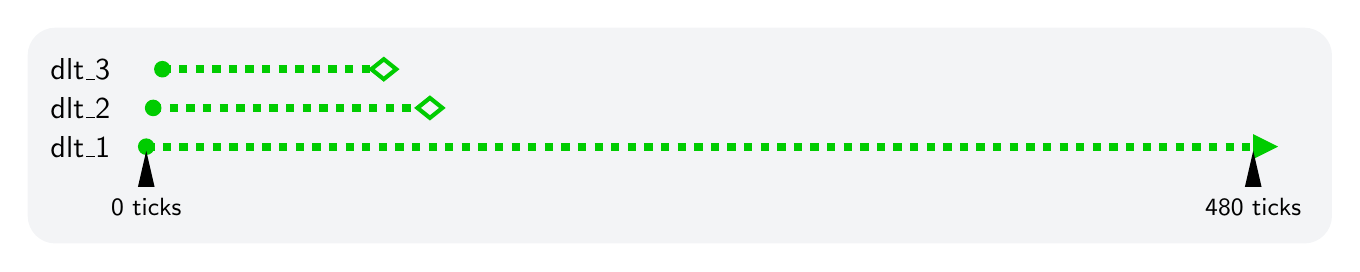
\begin{tikzpicture}[x=1pt,y=1pt,miter limit=4,font=\sffamily]
\definecolor{ts000000}{HTML}{000000}
\definecolor{ts00CC00}{HTML}{00CC00}
\definecolor{tsF3F4F6}{HTML}{F3F4F6}
\begin{scope}[shift={(16,16)}]
\path[rounded corners=10pt,fill=tsF3F4F6] (0,0) rectangle (471.3088,77.9766);
\path[draw=ts00CC00,line width=3pt,dash pattern=on 3pt off 3pt] (42.8501,34.9766) -- (442.8501,34.9766);
\path[fill=ts00CC00] (42.8501,34.9766) circle[radius=3];
\path[fill=ts00CC00] (451.8501,34.9766) -- (442.8501,39.4766) -- (442.8501,30.4766) -- cycle;
\path[draw=ts00CC00,line width=3pt,dash pattern=on 3pt off 3pt] (45.3501,48.9766) -- (140.8501,48.9766);
\path[fill=ts00CC00] (45.3501,48.9766) circle[radius=3];
\path[draw=ts00CC00,line width=1.5pt] (140.8501,48.9766) -- (145.3501,52.5766) -- (149.8501,48.9766) -- (145.3501,45.3766) -- cycle;
\path[draw=ts00CC00,line width=3pt,dash pattern=on 3pt off 3pt] (48.6834,62.9766) -- (124.1834,62.9766);
\path[fill=ts00CC00] (48.6834,62.9766) circle[radius=3];
\path[draw=ts00CC00,line width=1.5pt] (124.1834,62.9766) -- (128.6834,66.5766) -- (133.1834,62.9766) -- (128.6834,59.3766) -- cycle;
\path[fill=ts000000] (42.8501,33.4766) -- (39.8501,20.4766) -- (45.8501,20.4766) -- cycle;
\path[fill=ts000000] (442.8501,33.4766) -- (439.8501,20.4766) -- (445.8501,20.4766) -- cycle;
\node[anchor=base west,inner sep=0,font=\sffamily\fontsize{11}{12.8047}\selectfont,text=ts000000] at (8,59.1685) {dlt\_3};
\node[anchor=base west,inner sep=0,font=\sffamily\fontsize{11}{12.8047}\selectfont,text=ts000000] at (8,45.1685) {dlt\_2};
\node[anchor=base west,inner sep=0,font=\sffamily\fontsize{11}{12.8047}\selectfont,text=ts000000] at (8,31.1685) {dlt\_1};
\node[anchor=base,inner sep=0,font=\sffamily\fontsize{9}{10.4766}\selectfont,text=ts000000] at (42.8501,10.1226) {0 ticks};
\node[anchor=base,inner sep=0,font=\sffamily\fontsize{9}{10.4766}\selectfont,text=ts000000] at (442.8501,10.1226) {480 ticks};
\end{scope}
\end{tikzpicture}
\end{document}
